\documentclass{book}

\usepackage[subpreambles=false]{standalone}

%%%%%%%%%%%%%%%%%%%%%%%%%%%
% Silence warning messages
\usepackage{silence}
\WarningsOff[scrlayer-notecolumn]
\WarningsOff[biblatex]

%%%%%%%%%%%%%%%%%%%%
% Commenting

%\usepackage[author=Lyndon]{pdfcomment}
%\newcommand{\pdfcomment}[1]{} %ignore all comments

%\usepackage{todonotes}
%\newcommand{\pdfcomment}{\todo}


%%%%%%%%%%%%%%%%%%%%
% Tables
\usepackage{booktabs}

%%%%%%%%%%%%%%%%%%%
% Fonts
\usepackage{tgadventor} %sans
\usepackage{tgpagella}  %serif
\usepackage{inconsolata} %mono
\usepackage[T1]{fontenc}

\usepackage{microtype}
\usepackage[all]{nowidow}
%%%%%%%%%%%%%%%%%%%%%%%
% Styling
\setcounter{secnumdepth}{4}
\setcounter{tocdepth}{2}

\usepackage{placeins}



%%%%%%%%%%%%%%%%%%%
% Math
\usepackage{amsmath, amssymb, stmaryrd, mathtools}
\DeclareMathOperator*{\argmin}{argmin}
\DeclareMathOperator*{\argmax}{argmax}

\usepackage{xparse,xstring,etoolbox}
% crossref this against notation section
\newcommand{\vv}[1]{\tilde{#1}} % vector
\newcommand{\seq}[1]{\mathcal{#1}} % sequence
\newcommand{\set}[1]{\mathbb{#1}} % set

%%%%%%%%%
% Indexing/sequence indexing
\newcommand{\seqind}[2]{#1^{#2}} % seqence index
\newcommand{\ind}[2]{#1_{#2}} % indexed
\newcommand{\disamb}[2]{#1^{\mathrm{#2}}} %disambiguated

%% Smart indexing and naming
\newcommand{\ifupper}[3]{
    \normalexpandarg
	\exploregroups
	\StrCount{ABCDEFGHIJKLMNOPQRSTUVWXYZ}{#1}[\uppercount]
	\ifnumgreater{\uppercount}{0}{#2}{#3}
}

%smart index
\DeclareDocumentCommand{\ii}{u{_} m}{
	\ifupper{#1}%
	{% just a single uppercase character, i.e. a matrix
		  %make sure the index is the right length
		\StrCount{#2}{,}[\indcount]
		\ifnumgreater{\indcount}{0}
		{ % Got multiple indexes so all good
		 	\ind{#1}{#2}
		}
		{ % Only 1 index so grab the column
		 	\ind{#1}{{:,#2}}
		}
	}%
	{% Not just a single upper case character
		\ind{#1}{#2}
	}
}

\DeclareDocumentCommand{\nn}{u{_} m}{
	\seqind{#1}{#2}
}

\DeclareDocumentCommand{\dd}{u{_} m}{
	\disamb{#1}{#2}
}

% Index of a vector
\DeclareDocumentCommand{\iv}{u{_} m}{\ii{\vv #1}_{#2}}
\DeclareDocumentCommand{\dv}{u{_} m}{\dd{\vv #1}_{#2}}
\DeclareDocumentCommand{\nv}{u{_} m}{\nn{\vv #1}_{#2}}

%exp
\let\oldexp\exp
\renewcommand{\exp}[1]{\oldexp \left( #1 \right)}
\newcommand{\exptwo}[1]{\oldexp_2 \left( #1 \right)}

\newcommand{\softmax}{\mathrm{smax}}

\DeclareMathOperator*{\expectedop}{\mathbb{E}}
\DeclareDocumentCommand{\expected}{u{_} m}{
	\expectedop\limits_{\mathrlap{#2}}
}

%%%%%%%%%%%%%%%%
%Graphics
\usepackage{tikz}
\usetikzlibrary{positioning, fit,  shapes.geometric}
\usepackage{ifthen}
\usepackage{etoolbox}

\tikzset{
	backgroundcolor/.style ={fill=white},
	every node/.append style={
		minimum height=7mm,
	},
	labe/.append style={
		%Blue,
		align = center,
		backgroundcolor,
		fill opacity=0.6,
		text opacity=1,
		font={\footnotesize\itshape}	
	},
	layer/.append style={
		draw,
		align = center,
		minimum height=7mm,
	},
	tight/.append style={
		inner sep=0.2mm,
	},
	lookupbox/.append style={
		draw=none,
		append after command={
		       	[shorten <= -0.5\pgflinewidth]
		       	([shift={(-1.5\pgflinewidth,-0.5\pgflinewidth)}]\tikzlastnode.north east)
		       	edge([shift={( 0.5\pgflinewidth,-0.5\pgflinewidth)}]\tikzlastnode.north west) 
		       	([shift={( 0.5\pgflinewidth,-0.5\pgflinewidth)}]\tikzlastnode.north west)
		       	edge([shift={( 0.5\pgflinewidth,-1.5\pgflinewidth)}]\tikzlastnode.south west)            
		       	([shift={( -1.5\pgflinewidth,+0.5\pgflinewidth)}]\tikzlastnode.south east)
		       	edge([shift={(-1.5\pgflinewidth,-0.5\pgflinewidth)}]\tikzlastnode.north east)
		},
		inner sep=0.7mm,
		outer sep=0mm,
		minimum width=25mm
	}
}

\usepackage{pgfplots}
\pgfplotsset{compat=1.14}
\pgfplotsset{sideplot/.append style={
		width=\notescolwidth,
		domain=-10:10,
		samples=101,
		smooth,
		enlarge y limits={abs=2},
		axis lines=middle,
		xlabel  = $z$,
		ylabel  = $y$,
	},
	equ/.append style={
		color=blue,
		thick,
		mark=none
	}
}

% Function  For a plot 
% it  needs to be declared in preamble because of how \makenote* interacts with multiple files
\def\errorsurface(#1,#2){(0.5*#1 + 0.7*#2 + sin(deg(1.5*#1 + #2^2)))^2}


\usepackage{graphicx}
\graphicspath{{./figs/}, {./}, {./figs/chaptersentencerrepr/}, {./figs/chapterintromachinelearning/}, {./figs/chapterwordrepr/}}
\usepackage{adjustbox}


%%%%%%%%%%%%%%%%%%%
% Refs
\usepackage{cleveref}

\addbibresource{master.bib}

%%%%%%%%%%%%%%%%%%%%
% Formatting

% for examples from natural language space.
\newcommand{\natlang}[1]{\ifmmode \text{``\texttt{#1}''} \else {``\texttt{#1}''}\fi}
% \ifmmode ``trick'' from https://tex.stackexchange.com/a/15194/5834

%%%%%%%%%%%%%%%%%%%%%


\begin{document}
%%%%%%%%%%%%%%%%%%%%%%%%
\begin{titlepage}
\newgeometry{margin=1in}
\centering

{
	\Huge \sffamily 
	On the surprising capacity\\
	of linear combinations of embeddings\\
	for natural language processing\\
}
\vspace{1cm}
{\large Lyndon White\\
	{\normalsize BCM in Computation and Pure Mathematics; \\
	BE in Electrical and Electronic Engineering\\
	}
}
{\large\today\\}
\vspace{2cm}
\includegraphics[width=.50\linewidth]{figs/uwa}
\vfill
{
		\large
	This thesis is presented for the degree of\\
	Doctor of Philosophy\\
	of The University of Western Australia\\
}
\vspace{3cm}
\restoregeometry
\end{titlepage}
%%%%%%%%%%%%%%%%%%%%%%%%%%%%%%%%%%%%%%%%%%%%%%%%%



% See the structure of https://api.research-repository.uwa.edu.au/portalfiles/portal/9709033/THESIS_DOCTOR_OF_PHILOSOPHY_KHAN_Salman_Hameed_2016_Part_1.PDF


%%%%%%%%%%%%%%%%%%%%%%%%%%%%%%%%%%%%%%%%%%%%%%%%%%%
\cleardoublepage
\section*{Thesis Declaration}
\vskip 0.8cm
\begin{flushleft}
	I, Lyndon White, certify that:
	\vskip 0.5cm 
	This thesis has been substantially accomplished during enrolment in the degree.
	\vskip 0.25cm
	This thesis does not contain material which has been accepted for the award of any other degree or diploma in my name, in any university or other tertiary institution.
	\vskip 0.25cm
	No part of this work will, in the future, be used in a submission in my name, for any other degree or diploma in any university or other tertiary institution without the prior approval of The University of Western Australia and where applicable, any partner institution responsible for the joint-award of this degree.
	\vskip 0.25cm
	This thesis does not contain any material previously published or written by another person, except where due reference has been made in the text. 
	\vskip 0.25cm
	The work(s) are not in any way a violation or infringement of any copyright, trademark, patent, or other rights whatsoever of any person.
	\vskip 0.25cm
	The work described in this thesis was partially funded by 
	Australian Research Council grants DP150102405 and LP110100050;
	and by a Australian Government Research Training Program (RTP) Scholarship.
	\vskip 0.25cm
	This thesis contains published work and/or work prepared for publication, some of which has been co-authored. 
	\vskip 0.5cm

	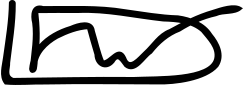
\includegraphics[height=2\baselineskip]{signatures/white}
	\vskip 0.15cm
	Lyndon White\\
	\today
\end{flushleft}



%%%%%%%%%%%%%%%%%%%%%%%%%%%%%%%%%%%%%%%%%%%%%%%%%%%%%%

{% Dedication
	\cleardoublepage
	\thispagestyle{empty}
	\vspace*{\stretch{1}}
	\centering
	{
		In memoriam of\\
		Laurie White\\
		\emph{1927--2018}\\
	}
	\vspace{\stretch{3}}
	\clearpage
}



%%%%%%%%%%%%%%%%%%%%%%%%%%%%%%%%%%%%%%%%%%%%%%%%%%%
\chapter*{Abstract}
As Webster's classic 1900 text \textit{``English: Composition and Literature''} states
``A sentence is a group of words expressing a complete thought.''
People use natural language to represent thoughts.
Thus the representation of natural language, in turn, is of fundamental importance in the field of artificial intelligence.
Natural language understanding is a research area which  revolves around how to represent text in a form that an algorithm can manipulate in such a way as to mimic the ability of a human to truly understand the text's meaning.
In this dissertation, we aim to extend the practical reach of this area,
by exploring a commonly overlooked method for natural language representation: linear combinations (i.e. weighted sums) of embedded representations.
This dissertation is organised as a collection of research publications:
 with our novel contributions published in conference proceedings or journals;
 and with a comprehensive literature review published as part of a book.

When considering how to represent English input into a natural language processing system,
a common response is to view it as a sequential modelling problem: as a discrete time-series of words.
A more complex alternative is to base the input model on the grammatical tree structures used by linguists.
But there are also simpler models: systems based on just summing the word embeddings.
Word embeddings are dense vector representations of words, generally learned as part of a neural network or related system.
They are commonly available pretrained, and are used in a variety of systems for different tasks to those they were originally trained for as a form of transfer learning.
On a variety of tasks, simply summing these word embeddings work very well -- often better than the more complex models.
This dissertation examines these linear combinations of embeddings for natural language understanding tasks.

In brief, it is found that a sum of embeddings is a particularly effective dimensionality-reduced representation of a bag of words.
The dimensionality reduction is carried out at the word level via the implicit matrix factorization 
on the collocation probability matrix.
It thus captures into the dense word embeddings the key features of lexical semantics:
words that occur in similar contexts have similar meanings.
We find that summing these representations of words gives us a very useful representation of structures built upon words: such as sentences, phrases, and word senses.

A limitation of the sum of embedding representation is that it is unable to represent word order.
This representation does not capture any order related information; unlike for example a recurrent neural network.
Recurrent neural networks, and other more complex models, are outperformed by sums of embeddings in tasks where word order is not highly significant.
It is found that even in tasks where word order does matter to an extent, the improved training capacity of the simpler model still means that it performs better than more complex models.
This limitation thus impacts surprisingly little.

%%%%%%%%%%%%%%%%%%%%%%%%%%%%%%%%%%%%%%%%%%%%%%%%%%%%%%%%%%%%%%%
\chapter*{Acknowledgements}
I must begin by expressing my gratitude towards my supervisors,
Prof. Roberto Togneri, Dr Wei Liu, and Winthrop Prof. Mohammed Bennamoun.
I am very fortunate to have such attentive supervisors,
who have supported me in my endeavours.
This thesis would not be here without their on-going support and advise.

Further, I wish to more generally thank the staff and faculty from the departments of electrical engineering and of computer science who've helped me during this process.

I would like to express how much I enjoyed working with Naeha Sharif on several projects.
I look forward to reading her thesis in a few years time.



This research was supported by an Australian Government Research Training Program (RTP) Scholarship.
The lack of which no doubt would have resulted in my expiration,
and the attendant adverse consequences on the completion of this dissertation.
It was also supported by funding from Australian Research Council grants DP150102405 and LP110100050.

During my research computing hardware and  power was provided due to the support of 
the National eResearch Collaboration Tools and Resources project (Nectar),
Nvidia, and the UWA University Computer Club (UCC).

I also to acknowledge the support and assistance I've received from my open-source collaborators and compatriots in the JuliaLang community.
In particular: Chris Rackauckas, Chrisof Stocker, and Jon Malmaud; though I could easily list a dozen more.
One could not ask for a more collegial online community of academics and programmers.

I am grateful for the ongoing support and companionship of my friends and family.
In particular, my good friend Roland Kerr, who began his Research Masters at the same time as I was beginning my PhD.

Lastly I must thank my darling wife, Isobel, who has supported me constantly;
and has always forgiven me when I am home hours late after just doing ``one last thing''.


\chapter*{Authorship declaration}



\section*{Publications}
%\begin{flushleft}

This thesis contains work that has been published and/or prepared for publication.




\DeclareDocumentCommand{\publication}{m m %
	O{Devised problem. Designed and implemented algorithms. Conducted experiments. Created figures. Wrote publication. Supervisors reviewed and provided useful feedback for improvement.} %
}{
	\begin{flushleft}
		\vskip 0.5cm
		\textbf{Details of the work:} \\
		\completecite{#2}\\
		
		
		\textbf{Location in thesis:} \Cref{#1}\\
		\textbf{Student contribution to work:} \\
		#3
		\\
	\end{flushleft}
}


\publication{LitRev}{NRoNL}[Determined content. Created figures. Wrote book. Supervisors reviewed and provided useful feedback for improvement.]
\publication{SentVecMeaning}{White2015SentVecMeaning}
\publication{ColorEst}{White2018ColorEst}
\publication{RefittingSenses}{WhiteRefittingSenses}
\publication{NovelPerspective}{novelperspective}
\publication{BOWgen}{White2015BOWgen}
\publication{SOWE2Sent}{White2016a}
\publication{DataDeps}{DataDeps}[Primary author of software. Created figures. Wrote publication. Supervisors reviewed and provided useful feedback for improvement.]
\publication{DataDepsGenerators}{DataDepsGenerators}[Original author of software. Provided direction, guidance, and code review for its enhancement. Wrote publication.]
\publication{Embeddings}{EmbeddingsPackage}[Original and primary author of software. Wrote publication.]
\publication{TensorFlow}{TensorFlowJulia}[Co-maintainer and second highest contributor to the software. Co-wrote publication.]


\section*{Permission to use work in thesis}
The coauthors signing below give permission to use the aforementioned works
in this dissertation,
and certify that the student's statements regarding their contribution to the respective co-authored works listed above are correct.


\vspace{1cm}



\DeclareDocumentCommand{\permission}{m O{\null} m m}{\
	\vskip 0.5cm
	\large
	\textbf{#1:}\\
	\emph{#2}
	\hfill
	\makebox(0,0){\raisebox{1.5\baselineskip}{\includegraphics[height=2\baselineskip]{#3}}}
	\hspace{3cm}
	#4
	\\
}

\permission{Roberto Togneri}[Primary Supervisor]{signatures/togneri}{04/10/18}
\permission{Wei Liu}[Supervisor]{signatures/liu}{04/10/18}
\permission{Mohammed Bennamoun}[Supervisor]{signatures/bennamoun}{04/10/18}
\permission{Sebastin Santy}{signatures/santy}{24/09/18}
\permission{David Ellison}{signatures/dellison}{02/10/18}
\permission{Jonathan Malmaud}{signatures/malmaud}{24/09/18}



%%%%%%%%%%%%%%%

\end{document}
